\cotefile{69}
\scanpage{3}

% head
\mspage{1}
\uline{Th.} Soit $S$ un graphe tel que

% ll. 2–4
\[
\begin{aligned}
\text{a)}\quad &\operatorname{card} S=27\\
\text{b)}\quad &\forall s\in S,\quad \operatorname{card} E(s)=10\qquad
 (E(s)=\{t\in S\mid t\text{ lié à }s\}\\
\text{c)}\quad &\forall s,t\in S,\quad s,t\text{ liés},\quad
 \exists!u\in S,\quad u\text{ lié à }s\text{ et }t.
\end{aligned}
\]

% l. 5
Alors (et alors seulement) $S$ est un graphe cubique.

% ll. 6–7
\uline{Dém} \unsure{Soit|Soient} $u\in S$, \deleted{$v\in E(s)$} ($\operatorname{card}S\geq27$ !) $v\in E(u)$ i.e. $v$ lié à $u$ ($\operatorname{card} E(u)=10$), $w\in S$ tel que $w$ lié à $u$ et $v$ (axiome c).

% l. 8
On dit que $T=\{u,v,w\}$ est un ``triangle''.

% ll. 9–10
\uline{Lemme 1} Tout $s\in S-\inserted{\unsure{(S^*=\{u,v,w\})|(\{u,v,w\})|\{u,v,w\}=S^*}}$ est lié à un et un seul des él. $u,v,w$ [ i.e. $S^*=S-\{u,v,w\}$ est \uline{réunion} \uline{disj.} de $E(u)^*=S^*\cap E(u),E(v)^*,E(w)^*$ (ch. un de cardinal 8)

% ll. 11–13
Comme $\operatorname{card} E(u)=10$, \deleted{\unsure{si on|tiens}} on a $\operatorname{card}\overbrace{E(u)\cap S^*}^{E(u)^*}=8$ car $E(u)\cap S^*=E(u)-\{v,w\}$, de même \deleted{card} $\overbrace{E(v)\cap S^*}^{\unsure{E(u)^*|E(v)^*}},\ \overbrace{E(w)\cap S^*}^{E(w)^*}$ sont de cardinal 8. Or par c), $E(u)\cap E(v)=\{w\}$ donc

% ll. 14–18
$E(u)^*\cap E(v)^*=\varnothing$ et de $=$ pour les autres 2 couples, donc $E(u)^*,E(v)^*,E(w)^*$ disjoints, donc la \deleted{\unsure{somme}}\inserted{réunion} est de cardinal \deleted{\unsure{24}} $3\times8=24$. Comme $S^*$ est de cardinal $27-3=24$ par a), on trouve que $S^*$ est réunion (disjointe) des $E(u)^*,E(v)^*,E(w)^*$, cqfd.

% ll. 19–20
\uline{Lemme} 2 $\forall x\in \deleted{\unsure{E(u)^*}}S^*$, $\exists!u'\in E(u)^*$ lié à $u$. (De $=$ pour $v,w$). / En effet, \deleted{\unsure{l'unicité est bien|l'unicité}}\inserted{\unsure{c'est une|n'est qu'une|des liés}} reformulation de c)

% ll. 21–23
\uline{Corollaire} $\exists!\sigma=\sigma_T:S\longrightarrow S$ tel que $\sigma_{\unsure{t|T}}$ laisse $u,v,w$ et que $\forall x\in S^*=S-\{u,v,w\}$, $\sigma_T(x)$ soit lié à $x$ et $x$ et $\sigma_{\unsure{t|T}}(x)$ liés au $=$ sommet $u,v,w$ de $T$.

% lower left, beside corollary
\figure{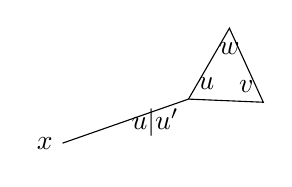
\begin{tikzpicture}[x=1cm,y=1cm]
\draw (0,0) -- (1.60,.56) -- (2.12,1.46) -- (2.55,.52) -- (1.60,.56);
\node[left] at (0,0) {$x$};
\node[below left] at (1.60,.56) {$\unsure{u|u'}$}; \node[above right] at (1.60,.56) {$u$};
\node[below] at (2.12,1.40) {$w$}; \node[above left] at (2.55,.52) {$v$};
\end{tikzpicture}}

% l. 24
Ainsi, chaque $E(u)^*,E(v)^*,E(w)^*$ se décompose \unsure{par|en} 4 couples de \inserted{pts liés}

% ll. 25–28
\uline{Lemme} 3 Soit $x\in E(u)^*$. Alors $\operatorname{card} E(x)\cap E(v)^*=4$. Si $x\in E(u)^*$, $y\in E(v)^*$, et si $x$ et $y$ liés, $x$ et $\sigma_t(y)$ non liés (et inversement.) En d'autres termes, $E(x)\cap E(v)^*$ contient un \unsure{élmt|élément} et un seul, dans chaque paire de sommets liés de $E(v)^*$.

% ll. 29–31
\uline{Dém} Si $x$ est lié à $y$, il ne peut être lié à $\sigma_t y$, sinon $\{y\text{ et }\sigma_t(y)\}$ serait \unsure{arête|côté} de \uline{deux} triangles distincts $\{v,y,\sigma_t(y)\}$ et $\{x,y,\sigma_t(y)\}$. \deleted{\unsure{Si $x$ et $\sigma_T y$ non|de $x$ et $\sigma_T(y)$}} \deleted{\unsure{Il faut exhiber}} \deleted{\unsure{les éléments cherchés}.}
% archive sheet number: 2
\scanpage{4}

% ll. 1–2
\mspage{2}
\[
\begin{aligned}
\text{Considérons}\quad A_x&=E(x)\cap\deleted{\unsure{S}}\{S^*-\sigma_t(x)\}=E(x)\cap(E(v)^*\cup E(w)^*)\\
&=E(x)-\{u,\sigma(x)\}
\end{aligned}
\]

% ll. 3–8
son cardinal est $10-2=8$ par b), \deleted{supposons que} : il se décompose en réunion disjointe de $E(\deleted{\unsure{y}}x)\cap E(v)^*=A_{\unsure{u|v}}$ et $E(x)\cap E(w)^*=A_w$, supposons que l'un \deleted{des deux soit} \deleted{\unsure{$A_v$ soit (dans limite)|$A_v,A_w$ (disons $A_w$)}} de cardinal $\ne4$, p. ex. $>4$ (sinon on intervertit $v$ et $w$). Alors $\exists\,y,y'$ liés dans $E(v)^*$ qui sont liés \unsure{au|à un} $=$ $x$, absurde on a vu.

% ll. 9–10
\uline{Corollaire} Si $x\in E(u)$, $y\in E(v)$ sont liés, $\sigma_{\unsure{t|T}}(x)$ et $\sigma(y)$ sont liés (et inv.)

% ll. 11–12
Si $x$ lié à $y$, $x$ non lié à $\inserted{y'=}\sigma_t(y)$, donc $\sigma_t(x)$ lié à $y'$, cqfd.

% l. 13
\uline{Corollaire} $\sigma_T=\sigma$ est un autom. de $S$.

% left beside cancelled lemma
\margin{\uline{NB}}

% ll. 14–18, crossed block
\deleted{\uline{Lemme 4} Soient $x,y\in E(u)^*$ non liés. Alors
\[
\begin{aligned}
&\operatorname{Card} E(x)\cap E(y)\cap E(v)^*=2.\\
&\text{i.e.}\quad \operatorname{card} w_x
\end{aligned}
\]
\uline{Dém} S'il était $\ne2$, on peut supposer qu'il est $>2$ [ quitte à remplacer \unsure{$x$|$y$} par $\sigma(y)$}

% left of cancelled proof
\figure{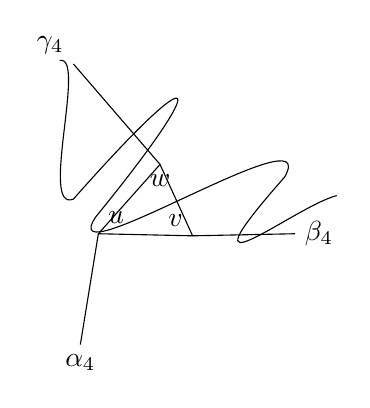
\begin{tikzpicture}[scale=.88]
\draw (0,-1.6) node[below] {$\alpha_4$} -- (.26,0) -- (1.15,1) -- (1.62,-.03) -- (.26,0);
\draw (1.15,1) -- (-.1,2.45) node[above left] {$\unsure{\gamma_4}$};
\draw (1.62,-.03) -- (3.1,0) node[right] {$\beta_4$};
\node[above right] at (.26,0) {$u$}; \node[above left] at (1.62,-.03) {$v$}; \node[below] at (1.15,1) {$w$};
\draw[thin] (-.3,2.5) .. controls (.1,2.6) and (-.6,.3) .. (-.1,.5) .. controls (1.8,2.65) and (1.9,2.3) .. (.22,.24) .. controls (-.4,-.7) and (3.5,1.8) .. (2.95,.82) .. controls (1.3,-1.05) and (3.1,.4) .. (3.7,.55);
\end{tikzpicture}}

% right of crossed block
\margin{\unsure{Introduire|Int. décrire|Introduisons} $P_u=E(u)^*/\sigma$ etc et $w_v(x)=\text{image de } E(x)\cap E(v)^*$ dans $P_v$, avec $w_v(\sigma x)=\unsure{\complement|C}w_v(x)$.}

% ll. 19–20
Soient $x,y\in\deleted{\unsure{S^*}}E(u)$, considérons

% ll. 19–20 right
\[
\begin{aligned}
w_v(x)&=E(x)\cap E(v)^*\\
w_v(y)&=E(y)\cap E(v)^*
\end{aligned}
\]

% ll. 21–23
\deleted{et une} \deleted{donc} on peut considérer $w_v(y)$ et $w_v(x)$ comme 2 sections de $E(v)^*$ sur $P_v=E(v)^*/\mathbb F_2$, donc leur différence est un élmt \deleted{\illegible{1}}.

% l. 24
\[
\delta_v(x,y)\in\mathbb F_2(P_v)
\]

% right of l. 24
\margin{\uline{NB} $\delta_v(x,\sigma(y))=\delta_v(\sigma x,y)=\delta_v(x,y)+\mathbb{1}_v$ \unsure{fonction} cte de v. 1 sur $P_v$}

% ll. 25–26
\[
\text{Donc}\quad
\left\{\begin{aligned}
\operatorname{supp}\delta_v(x,y)\deleted{\unsure{y}}&=\{\beta\in P_v\mid w_v(x)\cap\beta\ne w_v(y)\cap\beta\}\\
P_v-\operatorname{supp}\delta_v(x,y)&=\{\beta\in P_v\mid w_v(x)\cap\beta=w_v(y)\cap\beta\}=\text{image de}\\[-2pt]
&\hspace{2cm}w_v(x)\cap w_v(y)\text{ dans }P_v
\end{aligned}\right.
\]

% ll. 27–29
\uline{Lemme 4} \deleted{$\operatorname{Card}\operatorname{supp}\delta_v(x,y)=2$} Supposons $x,y\in E(u)^*$, $x$ et $y$ \uline{non liés} alors $\operatorname{Card}\operatorname{Supp}\delta_v(x,y)=2$ [ i.e. $\operatorname{card}\underbrace{w_v(x)\cap w_v(y)}_{E(x)\cap E(y)\cap E(v)^*}=2$ ]

% ll. 30–31
Sinon, ce cardinal serait $>2$ ou $<2$, et quitte à remplacer $y$ par $\sigma(y)$, on pourrait supposer
% archive sheet number: 3
\scanpage{5}

% l. 1
\mspage{\textcircled{3}}
qu'il est $>2$. Soient \deleted{donc}\inserted{d'abord} $s,t\in E(v)^*$ liés, \inserted{\unsure{ts deux|tous deux}} à $u$ et à $v$.

% ll. 2–3
a) Soient $x\in E(u)^*$, $s\in E(v)^*$, $x$ et $s$ liés. Soit $\unsure{\zeta|z|\xi}\in\deleted{\unsure{E(s)^*}}$ lié à $x$ et $s$. Alors \unsure{$\zeta\in E(w)^*$|$\xi\in E(v)^*$}

% ll. 3–6
\uline{Lemme 5} b) Soient $x,y\in E(u)^*$, $s,t\in E(v)^*$, $x$ et $y$ liés \inserted{(à la fois)} à $s$ et à $t$. [ donc par lemme 3, $x$ et $y$ non liés, $s$ et $t$ non liés). \deleted{\unsure{Soit $\in S$|Soit}} Soient $\zeta,\zeta'$ \deleted{\unsure{$\zeta$ tel}} tels que \deleted{$\unsure{\zeta,(x,s,\zeta)|\xi,(x,s)}$ et $(y,t,$} $\zeta$ lié à $x$ et $s$, $\zeta'$ lié à $y$ et $t$. Alors $\zeta,\zeta'\in E(w)^*$, et $\zeta,\zeta'$ liés.

% ll. 7–11
Démonstration du lemme 5. \deleted{Soit $x$} a) On a $\zeta\in S^*$ car $\zeta\ne u,v,w$ (car $u$ non lié à $s$, $v$ non lié à $x$, $w$ lié ni à $x$ ni à $s$) et $\zeta\notin E(u)^*$, sinon on aurait $\zeta=\sigma(u)$ et $\zeta$ \deleted{\unsure{$\zeta$}} non lié à $s$ par lemme 3, de $=$ $\zeta\notin E(v)^*$, donc $\zeta\in E(w)^*$.

% ll. 12–18
b) Comme $\{x,\unsure{\zeta,s|s,\zeta|\xi,s}\}$ est un triangle, $\zeta'$ est lié à un \deleted{\unsure{pt|et}}\inserted{sommet} et un seul de ce triangle. Or il n'est pas lié à $x$ (sinon $\{\zeta',t\}$ serait arête de deux triangles distincts $\{\zeta',t,x\}$ et $\{\zeta',t,y\}$) ni à $s$ (\deleted{sinon} raison symétrique) donc il est lié à $\zeta'$.

% left beside ll. 13–16
\figure{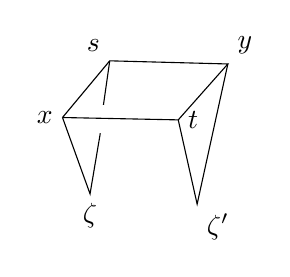
\begin{tikzpicture}[x=1cm,y=1cm]
\draw (0,0) node[left] {$x$} -- (.6,.72) node[above left] {$s$} -- (2.1,.68) node[above right] {$y$} -- (1.47,-.03) node[right] {$t$} -- (0,0);
\draw (0,0) -- (.35,-.97) node[below] {$\zeta$} -- (.48,-.20);
\draw (.52,.16) -- (.6,.72);
\draw (1.47,-.03) -- (1.71,-1.10) node[below right] {$\zeta'$} -- (2.1,.68);
\end{tikzpicture}}

% ll. 19–23
\uline{Dém. du lemme} 4 Supposons $x,y\in E(u)^*$ \inserted{$(x\ne y)$} liés à $s,t,r\in E(v)^*$ distincts. Considérons le triangle $\{x,s,\zeta\}$, donc (lem. 5a) $\zeta\in E(w)^*$, et si $\zeta'=\sigma(t)\in E(w)^*$, en vertu du lemme 5 b) \inserted{appliqué à $(x,y),(s,t)$} $\{\deleted{\unsure{\zeta}}y,t,\zeta'\}$ est un triangle, mais aussi $\{y,r,\zeta'\}$ en regardant $(x,y)\ (s,r)$. Donc

% left beside l. 22
\margin{$x\quad y\qquad s\quad t\quad r$}

% l. 24
$\{y,\zeta'\}$ appartiendrait à 2 triangles, absurde.

% ll. 25–30
\deleted{\uline{Lemme 6}}\inserted{Corollaire 1} Il existe une application \inserted{bijective, \unsure{c.v.c.|c.v., ce|canon.}} et une seule de $\Pi_{22}(P_u)$ dans $\Pi_{22}(P_{\unsure{v|w}})$ ($\Pi_{22}$ indique partitions de type $2,2$) telle que pour \unsure{tte|tout} \deleted{\unsure{partie à 2 élmts de}} \deleted{toute partie à} couple $x,y$ de pts non liés de $E(u)^*$, \deleted{la partition} on ait

% lower left at corollary
\margin{$\pi_u:E_u^*\longrightarrow\underset{\substack{\Vert\\ E_u^*/\mathbb F_2}}{P_u}$}

% bottom
\[
\begin{aligned}
c_{v,u}(\{\pi_u\{x,y\},\complement_{P_u}\pi_u\{x,y\}\}
&=\{\operatorname{supp}\delta_v(x,y),\operatorname{supp}\delta_v(x,y)+\mathbf{1}_{P_v}\}.
\end{aligned}
\]
% archive sheet number: 4
\scanpage{6}

% ll. 1–3
\mspage{\textcircled{4}}
Il faut montrer que le $2^{\mathrm{ième}}$ mb ne dépend que de la partition $\in\Pi_{22}(P_u)$, pas du choix de $(x,y)$. Pour ceci, on note

% ll. 4–5
a) Elle est indépendante par permutation de $x$ et $y$ \deleted{\unsure{c'est}} (car $\delta_v(x,y)=\delta_v(y,x)$)

% ll. 6–8
b) Elle ne change pas si on change $x$ et $\sigma(x)$ (ou aussi $y$ en $\sigma(y)$, ou $x$ en $\sigma(x)$ et $y$ en $\sigma(y)$) (car $\delta_v(\sigma x,y)=\delta_v(x,y)+1$)

% ll. 9–13
c) Si $x,y$ sont fixés, \deleted{\unsure{prenons|posons}}\inserted{posant (lemme 4)} \deleted{$s\ne t$} $\{s,t\}=\deleted{E(x)\cap E(y)\cap E(v)^*}E(x)\cap E(y)\cap E(v)^*$, donc \inserted{(id)} $\{x,y\}=E(s)\cap E(t)\cap E(u)^*$, \deleted{soient}\inserted{soit} $\{\unsure{\xi|z|x'},\eta\}=E(s)\cap E(\sigma(t))\cap E(u)^*$, alors $\pi_u(\{\xi,\eta\})=\complement_{P_u}\pi_u(\{x,y\})$, \deleted{\unsure{donc $x',y$|donc $x',y'$}} et $\{\xi,\eta\}$ donne donc lieu à la $=$ partition $\in\Pi_{2,2}(P_u)$ que $\{x,y\}$,

% ll. 14–19
mais à $\{\xi,\eta\}$ la recette \deleted{\unsure{préc.|prise}} de l'énoncé du corollaire associe la partition en $\pi_v(\underbrace{E(\xi)\cap E(\eta)\cap E(v)^*}_{\{s,\sigma(t)\}})$ et son complé\unsure{mentaire|mtaire}, qui \deleted{\unsure{sont}} égaux à $\underbrace{\pi_v\{s,t\}}_{\operatorname{supp}(\delta_v(x,y)+1)}$ et son complé\unsure{mentaire|mtaire} \unsure{---|\dots}

% l. 20
Énoncé plus fort :

% ll. 21–22
\deleted{\unsure{Cor}}\uline{Corollaire 2} Soit $\mathcal P'_2(E_u^*)$ l'ens des \deleted{couples}\inserted{parties à} 2 éléments de $E_u^*$ formés de deux él. non \uline{liés}.

% ll. 23–25
Soit $R_{u,v}$ la relation \deleted{entre} dans $\mathcal P'_2(E_u^*)\times\mathcal P'_2(E_v^*)$ : $R_{u,v}(\deleted{\unsure{\beta}}\alpha,\beta)\overset{\text{déf}}{\Longleftrightarrow}$ tt el. de $\alpha$ est lié à tt el. de $\beta$. Alors $R_{u,v}$ \inserted{définit} une bijection

% lower left, oblique
% slanted
\margin{\unsure{énoncé|énoncés|\deleted{Énoncé}} plus simple avec $R'_{uv}(\alpha,\beta)$ : tt él. de $\alpha$ \uline{non lié} à tt él. de $\beta$, $[\Longleftrightarrow R_{uv}(\sigma\alpha,\beta)\Longleftrightarrow R_{uv}(\alpha,\sigma\beta)]$ car les \unsure{applications|appl:ations} $\varphi'_{vu}:\mathcal P_2(E_u^*)\to\mathcal P_2(E_v^*)$ forment un syst. \uline{transitif} d'iso (comme on \unsure{le verra|verra} au lemme 6 ci-dessous)}

% ll. 26–27
de $\mathcal P'_2(E_u^*)$ sur $\mathcal P'_2(E_v^*)$, soit \deleted{$\varphi$}

% ll. 27–29
\[
\begin{aligned}
\widetilde\varphi_{vu}:\mathcal P'_2(E_u^*)&\longrightarrow\mathcal P'_2(E_v^*)\\
\widetilde\varphi_{vu}(\sigma\widetilde\alpha)&=\sigma\widetilde\varphi_{vu}(\widetilde\alpha)\\
\pi_v\widetilde\varphi_{vu}(\{x,\sigma y\})&=\complement_{P_v}\pi_v\varphi_{vu}(\{x,y\})
\end{aligned}
\]
% archive sheet number: 5
\scanpage{7}

% ll. 1–4, 6–7
\mspage{\textcircled{5}}
donc la partition définie par $\deleted{\unsure{\pi_u\{x,\sigma y|\pi_u(x,\sigma y}}\pi_v\varphi_{vu}(\{x,y\})$ ne change pas en remplaçant $x$ par $\sigma(x)$, (ou $y$ par $\sigma(y)$, ou les deux à la fois) donc ne dépend que de $\deleted{\unsure{\widetilde\alpha\rightarrow P_v|\pi_u\varphi}}\alpha=\pi_u(\{x,y\})\in\mathcal P_{\,2,2}(P_u)$ ; enfin, elle ne change pas si on remplace $\alpha$ par $\complement_{P_u}\alpha\dots$

% upper left, first two segments
\figure{\begin{tikzpicture}[x=.78cm,y=.70cm]
\fill (0,0) circle (1.4pt);
\node[below] at (0,-0.01) {$x$};
\node[below] at (0,-0.52) {$\binom{s}{t}$};
\fill (0.85,0) circle (1.4pt);
\node[below] at (0.85,-0.01) {$x'$};
\node[below] at (0.85,-0.52) {$\binom{s'}{t'}$};
\fill (2,0) circle (1.4pt);
\node[below] at (2,-0.01) {$y$};
\node[below] at (2,-0.52) {$\binom{s}{t}$};
\fill (2.85,0) circle (1.4pt);
\node[below] at (2.85,-0.01) {$y'$};
\node[below] at (2.85,-0.52) {$\binom{s'}{t'}$};
\draw[very thick] (0,0)--(.85,0) (2,0)--(2.85,0);
\end{tikzpicture}}

% upper left, second two segments
\figure{\begin{tikzpicture}[x=.78cm,y=.70cm]
\fill (0,0) circle (1.4pt);
\node[above] at (0,0) {$\zeta$};
\node[below] at (0,-0.12) {$\binom{s}{t'}$};
\fill (0.85,0) circle (1.4pt);
\node[above] at (0.85,0) {$\zeta'$};
\node[below] at (0.85,-0.12) {$\binom{s'}{t}$};
\fill (2,0) circle (1.4pt);
\node[above] at (2,0) {$\eta$};
\node[below] at (2,-0.12) {$\binom{s}{t'}$};
\fill (2.85,0) circle (1.4pt);
\node[above] at (2.85,0) {$\eta'$};
\node[below] at (2.85,-0.12) {$\binom{s'}{t}$};
\draw[very thick] (0,0)--(.85,0) (2,0)--(2.85,0);
\end{tikzpicture}}

% upper centre, joined pairs
\figure{\begin{tikzpicture}[x=.78cm,y=.70cm]
\fill (0,0) circle (1.4pt);
\node[below] at (0,-0.01) {$s$};
\node[below] at (0,-0.52) {$\binom{x}{y}$};
\fill (0.85,0) circle (1.4pt);
\node[below] at (0.85,-0.01) {$s'$};
\node[below] at (0.85,-0.52) {$\binom{x'}{y'}$};
\fill (2,0) circle (1.4pt);
\node[below] at (2,-0.01) {$t$};
\node[below] at (2,-0.52) {$\binom{x}{y}$};
\fill (2.85,0) circle (1.4pt);
\node[below] at (2.85,-0.01) {$t'$};
\node[below] at (2.85,-0.52) {$\binom{x'}{y'}$};
\draw[very thick] (0,0)--(.85,0) (2,0)--(2.85,0);
\draw (0,.19)--(.98,1.13)--(1.96,.18) (.85,.2)--(1.83,1.25)--(2.82,.18);
\end{tikzpicture}}

% upper centre right, cancelled pairs
\figure{\begin{tikzpicture}[x=.78cm,y=.70cm]
\fill (0,0) circle (1.4pt);
\node[below] at (0,-0.01) {$\unsure{u}$};
\node[below] at (0,-0.52) {$\binom{x}{\unsure{y''|y'}}$};
\fill (0.85,0) circle (1.4pt);
\node[below] at (0.85,-0.01) {$u'$};
\node[below] at (0.85,-0.52) {$\binom{x'}{y}$};
\fill (2,0) circle (1.4pt);
\node[below] at (2,-0.01) {$v$};
\node[below] at (2,-0.52) {$\binom{x}{y'}$};
\fill (2.85,0) circle (1.4pt);
\node[below] at (2.85,-0.01) {$v'$};
\node[below] at (2.85,-0.52) {$\binom{x'}{y}$};
\draw[very thick] (0,0)--(.85,0) (2,0)--(2.85,0);
\draw (0,.19)--(.98,1.13)--(1.96,.18) (.85,.2)--(1.83,1.25)--(2.82,.18);
\draw (0,.6) .. controls (0,-2.3) and (.1,1.3) .. (1.2,1.1) -- (.2,-1.7) -- (2.25,1.15) -- (.8,-1.75) -- (2.65,.75) .. controls (2,-1.9) and (1.9,.65) .. (3.06,.23) -- (2.68,-1.5) -- (.25,-1.48);
\end{tikzpicture}}

% ll. 8–10
\uline{\deleted{Corollaire}\inserted{Lemme} 6} $c_{wv}c_{vu}=c_{wu}$ --- donc les $c_{vu}$ etc définissent un syst. transitif d'iso entre les $\Pi_{22}(P_u),\Pi_{22}(P_v),\Pi_{22}(P_w)$

% ll. 11–13, crossed diagonally
\deleted{Soit $\{s,t\}=\unsure{\tau_{vu}|c_{vu}}\{x,y\}$ \inserted{$(x,y\in E(u)^*$ non liés)}. Soit $\zeta\in E(w)^*$ lié à $x$ et $s$, (lemme 5 a)), $\eta\in E(w)^*$ lié à $y,t$.}

% left of ll. 10–13
\figure{\begin{tikzpicture}[scale=.85]
\draw (0,.28)--(2.1,0)--(1.98,2.2);
\node[left] at (0,.22) {$x$}; \node[below] at (.25,.18) {$y$};
\node[right] at (2.1,0) {$s\quad t$};
\fill (1.98,2.67) circle(.8pt) node[above] {$w$};
\fill (.92,1.36) circle(.8pt) node[above] {$u$};
\fill (2.64,1.39) circle(.8pt) node[right] {$v$};
\end{tikzpicture}}

% l. 14
Cela \deleted{\unsure{résulte du|résulte}}\inserted{est inclus dans le} résultat plus précis

% ll. 15–16
\[
\begin{aligned}
\text{\uline{Corollaire}}\qquad
\widetilde\varphi_{wv}\widetilde\varphi_{vu}(\widetilde\alpha)&=\sigma(\widetilde\varphi_{wu}(\widetilde\alpha))\qquad\text{i.e.}\\
\widetilde\varphi_{wv}\widetilde\varphi_{vu}&=\sigma\widetilde\varphi_{wu}
\end{aligned}
\]

% ll. 17–19
\[
\begin{aligned}
\text{i.e.}\quad x,y\in E(u)^*&\quad x,y\text{ liés à }s,t\\
s,t\in E(v)^*&\quad s,t\text{ liés à }p,q\\
\{p,q\}\in E(w)^*&\quad\Longrightarrow xy\text{ liés à }\sigma p,\sigma q
\end{aligned}
\]

% lower left, first polyhedron
\figure{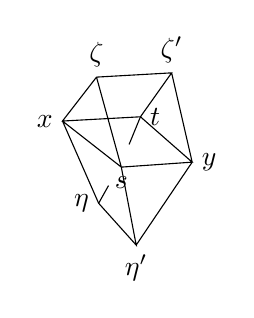
\begin{tikzpicture}[scale=.9]
\coordinate (x) at (0,1.2);\coordinate (t) at (1.1,1.26);\coordinate (y) at (1.83,.62);\coordinate (s) at (.83,.55);
\coordinate (z) at (.48,1.82);\coordinate (zz) at (1.54,1.88);\coordinate (h) at (.51,.04);\coordinate (hh) at (1.04,-.55);
\draw (x)--(z)--(zz)--(t)--cycle (x)--(s)--(y)--(t) (z)--(s)--(hh)--(h)--(x) (y)--(hh) (zz)--(y);
\draw (h)--(.65,.29) (t)--(.94,.87);
\node[left] at (x) {$x$}; \node[right] at (t) {$t$}; \node[right] at (y) {$y$}; \node[below] at (s) {$s$};
\node[above] at (z) {$\zeta$}; \node[above] at (zz) {$\zeta'$}; \node[left] at (h) {$\eta$}; \node[below] at (hh) {$\eta'$};
\end{tikzpicture}}

% lower left below first drawing, struck through
\figure{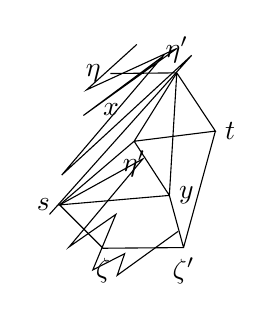
\begin{tikzpicture}[scale=.86]
\coordinate (a) at (.75,1.8);\coordinate (b) at (1.73,1.81);\coordinate (c) at (2.3,.95);\coordinate (d) at (1.62,0);
\coordinate (e) at (0,-.14);\coordinate (f) at (.64,-.78);\coordinate (g) at (1.83,-.77);\coordinate (h) at (1.10,.8);
\draw (a)--(b)--(c)--(h)--(e)--(d)--(b) (e)--(f)--(g)--(c) (g)--(d)--(h)--(b);
\node[left] at (e) {$s$};\node[right] at (c) {$t$};\node[left] at (a) {$\eta$};\node[above] at (b) {$\unsure{\eta'}$};
\node[above] at (.76,1.03) {$x$};\node[below] at (h) {$\eta'$};\node[right] at (d) {$y$};\node[below] at (f) {$\zeta$};\node[below] at (g) {$\zeta'$};
\draw (-.15,-.28)--(1.95,2.07)--(.03,.3)--(1.52,2.05)--(.35,1.18)--(1.73,2.17)--(.4,1.56)--(1.14,2.23)
 (0,-.14)--(1.23,.54)--(.14,-.76)--(.83,-.28)--(.49,-1.10)--(.96,-.86)--(.85,-1.18)--(1.75,-.53);
\end{tikzpicture}}

% ll. 20–23
Prouvons d'abord le lemme 6. Comme \unsure{ds|dans} lemme 5, complétons les triangles

% ll. 22–23
\[
\begin{aligned}
(x,s,\zeta),\ (y,t,\zeta')&\quad(\zeta,\zeta'\in E(w)^*\text{ sont liés})\\
(x,t,\eta),\ (y,s,\eta')&\quad(\eta,\eta'\in E(w)^*\text{ sont liés})
\end{aligned}
\]

% ll. 24–26
Alors $\zeta$ lié à $s$, \uline{non à $t$} (sinon $(\zeta,t)$ appartiendrait à 2 triangles de sommets $x,\zeta'$) de $=$ $\eta$ lié à $t$, non à $s$, donc cela montre que

% l. 27
\[
\{\pi_w(\{\zeta,\eta\}),\complement_{P_w}\pi_w(\{\zeta,\eta\})\}
=\unsure{\widetilde\varphi_{wv}|c_{wv}}(\pi_{\unsure{w|v}}\{s,t\},\complement\pi_w(\{s,t\})),
\]

% ll. 28–29
Mais aussi $\zeta$ lié à $x$, non à $y$, $\eta$ lié à $x$, non à $y$ donc $\{\pi_w(\{\zeta,\eta\}),\complement\pi_w(\{\zeta,\eta\})\}=c_{wu}'(\pi_u(\{x,y\}),\complement\pi_u(\{x,y\}))$
% archive sheet number: 6
\scanpage{8}

% ll. 1–5
\mspage{\textcircled{6}}
cqfd.

Ceci étant soient $p\ne q\in E(w)^*$ liés à $s,t$, on sait \inserted{donc} qu'ils sont non liés à $\zeta,\zeta',\eta,\eta'$ et non liés entre eux i.e. $E(w)^*=\{\zeta,\zeta',\eta,\eta',p,p',q,q'\}$, où $p'=\sigma p$, $q'=\sigma q$. On a $p$ non lié à $x$ (sinon $px$ appartiendrait à 2 triangles de sommets $s,t$)

% ll. 6–10
de $=$ $p$ non \unsure{lié|liée} à $y$, donc $p'$ lié à $x$ et $y$. de $=$ $q'$ lié à $x$ et $y$, i.e.
\[
\{p',q'\}=\widetilde\varphi_{wu}(\{x,y\})
\]
ce qui prouve le corollaire.

% left beside ll. 6–8
\figure{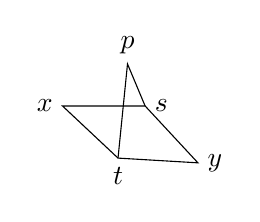
\begin{tikzpicture}[scale=.86]
\draw (0,0) node[left] {$x$} -- (1.22,0) node[right] {$s$} -- (2,-.84) node[right] {$y$} -- (.82,-.77) node[below] {$t$} -- cycle;
\draw (.82,-.77) -- (.96,.62) node[above] {$p$} -- (1.22,0);
\end{tikzpicture}}

% separator
\begin{center}\rule{2.2cm}{.35pt}\end{center}

% ll. 11–15
On identifie entre eux les $\Pi_{22}(P_u,P_v,P_w)$, soit $\unsure{J|\mathcal J|\sqsupset}$ de cardinal 3. [ Soit $V$ le \unsure{vectoriel|vectorl} de dim 2 sur $\mathbb F_2$ associé $(J=V^*)$ donc $P_u,P_v,P_w$ apparaissent comme des torseurs sous $V^*$. Soit $I=\{u,v,w\}$.

% ll. 16–18
\deleted{On a} Soit $\unsure{\widetilde{\mathscr T}|\widetilde\Gamma}$ l'ens des triangles $\subset S^*$, on voit que $\widetilde{\mathscr T}\xrightarrow{\sim}\prod_{\underbrace{x\in E(u)^*}_{\text{card. }8}}\underbrace{\unsure{w_v(u)|\omega_v(u)|\omega_v(x)}}_{\text{card }4}$ donc $\operatorname{Card}\widetilde{\mathscr T}=32$. Soit $\Gamma=\widetilde{\mathscr T}/\sigma$ (de cardinal 16)

% ll. 19–21
\uline{Lemme} 7 $\mathscr T\longrightarrow\underbrace{P_u\times P_v\times P_w}_{\text{cardinal }64=4.4.4}$ est : injectif, et \deleted{\unsure{$\mathscr T$}}\inserted{l'image de $\Gamma$} est un sous-torseur sous $\Psi(\unsure{W|V})\subset V\times V\times V$,

% l. 22
\[
(\Psi(V)=\{(x,y,z)\in V\times V\times V\mid x\unsure{+|-}y+z=0).
\]

% ll. 23–26
\uline{Dém} Soit $(x,s,\zeta),(y,t,\eta)$ deux triangles ayant $=$ image dans $P_u\times P_v\times P_w$. Quitte à appliquer $\sigma$ au $2^e$, \unsure{OPS|QPS} $y=x$. Alors $s$ et $t\in E(\unsure{u|v})^*$ liés à $x$ ne peut \deleted{être} satisfaire $t=\sigma s$, donc $t=s$, de $=$
% archive sheet number: 7
\scanpage{9}

% ll. 1–5
\mspage{\textcircled{7}}
$\unsure{\zeta|z|\xi}=\eta$, d'où l'injectivité. Montrons que $\Gamma$ est stable par les éléments de $N_u=\operatorname{Ker}(\Psi\xrightarrow{\mathrm{pr}_1}V)$ (donc aussi par $N_v$ et $N_w$) --- il s'ensuivra qu'il est stable par $\Psi\underset{\unsure{?|\gamma}}{=}N_u+N_v$, donc (étant de cardinal $16=\operatorname{card}\Psi$) c'est un torseur sous $\Psi$. \unsure{Cela|Ceci} équivaut au

% ll. 6–9
\uline{Corollaire} Soit $x\in E(u)^*$, $s\in E(v)^*$, $\zeta\in E(w)^*$ formant triangle. \deleted{Alors} Soit \deleted{\unsure{$q$}} $t\in E(v)^*$ \inserted{$t\ne s$} non lié à $s$, et lié à $\zeta$ (il y en a trois), et soit $\eta$ l'élmt de $E(w)^*$ distinct de $\zeta$ lié à $s,t$ (lemme 4). Alors

% l. 10
\[
\deleted{\unsure{\varphi}}(\pi_u(x),\pi_{\unsure{u|v}}(t),\pi_{\unsure{u|w}}(\eta))\in\operatorname{Im}(\Gamma\longrightarrow P_u\times P_v\times P_w),
\]

% ll. 11–13
\deleted{i.e. $\{x,\eta,t\}$ est un triangle, ou un} \deleted{Alors} plus précisément $(x,\sigma t,\sigma\eta)$ est un triangle.

% left of corollary
\figure{\begin{tikzpicture}[scale=.86]
\draw (0,1) node[above left] {$v$} -- (1.2,.74) node[right] {$w$} -- (.16,0) node[below] {$u$} -- cycle;
\draw (.32,.70)--(.61,.92);
\node at (-.12,2.25) {$\zeta$}; \node at (.36,2.25) {$\eta$};
\node at (2.45,.80) {$\unsure{t}$}; \node at (2.52,.47) {$s$}; \node at (-.2,-.90) {$x$};
\end{tikzpicture}}

% ll. 14–18
\uline{Dém} Comme $x$ est lié à $s$ et $\zeta$, liés resp. à $\eta$ et $t$, il ne peut être lié à $t$ ni $\eta$, donc il est lié à $\sigma t$ et $\sigma\eta$, qui sont liés entre eux (\deleted{qui} puisque $t$ et $\eta$ le sont) cqfd.

% left of demonstration
\figure{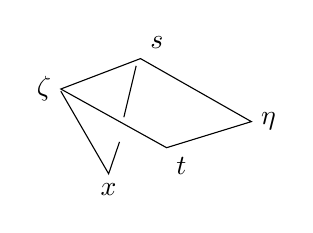
\begin{tikzpicture}[scale=.92]
\draw (0,.7) node[left] {$\zeta$} -- (1.10,1.12) node[above right] {$s$} -- (2.63,.25) node[right] {$\eta$} -- (1.46,-.11) node[below right] {$t$} -- cycle;
\draw (0,.67)--(.66,-.47) node[below] {$x$} -- (.81,-.03) (1.04,1.02)--(.87,.31);
\end{tikzpicture}}

% ll. 19–25
\uline{NB} La donnée de $V$ et du torseur $\Gamma$ sous $\Psi(\unsure{W|V})$ permet de réconstituer $P_u,P_v,P_w$ et la notion de ``triangles'' dans $P_u\times P_v\times P_w$. Il faut encore réconstituer les rev. à 2 feuillets $E(u)^*\inserted{=\widetilde P_u},E(v)^*\inserted{=\widetilde P_v},E(w)^*\inserted{=\widetilde P_w}$ de $P_u,P_v,P_w$, et le \unsure{revêmt|revêment|revêtement} à 2 feuillets $\unsure{\widetilde{\mathscr T}|\widetilde\Gamma}$, et les liens $\widetilde\Gamma\mathbin{-}\widetilde P_u$ etc sur $\Gamma\to P_u$ etc. $\big]$

\noindent ---
% archive sheet number: 8
\scanpage{10}

% ll. 1–6
\mspage{\textcircled{8}}
\uline{Épinglage}. Fixons un triangle $(\alpha_4,\beta_4,\gamma_4)\in\widetilde\Gamma$ ($\alpha_4\in E(u)^*,\beta_4\in E(v)^*,\gamma_4\in E(w)^*$). Alors $\Pi_{22}(P_u)$ s'identifie à $P_u-\{\pi_u(\alpha_4)\}$, de $=\dots$. Ordonnons $V^*$, donc les $P_u-\{\pi_u(\alpha_4)\}$ etc. Dans $\unsure{E_u(u)^*|E(u)^*}-\{\alpha_4\}$ sur $P_u-\{\pi_u(\alpha_4)\}$ il y a une section $\{\alpha_1,\alpha_2,\alpha_3\}$, définie par

% ll. 7–9
\diagram{\(\displaystyle
\mathrm I_0\left\{\begin{array}{lll}
\alpha_1,\alpha_2,\alpha_3\ (\text{et }\alpha_4)&\text{liés à }\beta_4&\text{; de }=\\
\beta_1\ \beta_2,\beta_3\ (\text{et }\beta_{\unsure{3|4}})&\rule{1.15cm}{.35pt}\quad\gamma_4&\\
\gamma_1\ \gamma_2\ \gamma_3\ (\text{et }\gamma_4)&\rule{1.15cm}{.35pt}\quad\alpha_4&
\end{array}\right.
\)}

% ll. 10–14
Ainsi, en termes d'un ordre total sur $J=V^*$ et d'un ordre total (ou \unsure{seulemt|seulement} un ordre circulaire) sur \deleted{\unsure{$\Delta$}}\,$I:\{u,v,w\}$, on a épinglé les 24 \inserted{$=2\times12=2\times(3\times4)$} él. de $S^*$ (\unsure{en plus} des $u,v,w$) par les $\alpha_i,\beta_i,\gamma_i$, $\alpha'_i=\sigma\alpha_i$, $\beta'_i=\sigma\beta_i$, $\gamma'_i=\sigma\gamma_i$.

% ll. 15–16
De (I) et lem 3, on déduit [0] $\alpha_i$ lié à $\alpha'_i$ / $\beta_i$ à $\beta'_i$ /, $\gamma_i$ à $\gamma'_i$.

% left linking I to I' and [0]
\figure{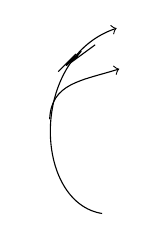
\begin{tikzpicture}[scale=.68]
\draw[->] (1,-2) .. controls (-.28,-1.8) and (-.38,.9) .. (1.27,1.46);
\draw[->] (.02,-.24) .. controls (.05,.44) and (.62,.48) .. (1.32,.70);
\draw (.18,.65)--(.51,.98)--(.33,.76)--(.61,1.03)--(.46,.85)--(.87,1.15);
\end{tikzpicture}}

% rows I prime
\diagram{\(\displaystyle
\mathrm I'\left\{\begin{array}{llll}
\alpha'_i\ \deleted{\unsure{\alpha_1,\alpha_2,\alpha_3}}&\text{liés à }\beta'_4,&\text{non à }\beta_4&\text{ni entre eux}\\
\beta'_i&\rule{.9cm}{.35pt}\quad\gamma'_4,&\text{non à }\gamma_4&\text{ni entre eux}\\
\gamma'_i&\rule{.9cm}{.35pt}\quad\alpha'_4,&\text{non à }\alpha_4&\text{ni entre eux}
\end{array}\right.
\)}

% rows I
\diagram{\(\displaystyle
\mathrm I\left\{\begin{array}{llll}
\alpha_i&\text{liés à }\beta_4,&\text{non à }\beta'_4&\text{ni entre eux}\\
\beta_i&\rule{1cm}{.35pt}\quad\gamma_4&\rule{.85cm}{.35pt}\quad\gamma'_4&\rule{1.4cm}{.35pt}\\
\gamma_i&\rule{1cm}{.35pt}\quad\alpha_4&\rule{.85cm}{.35pt}\quad\alpha'_4&\rule{1.4cm}{.35pt}
\end{array}\right.
\)}

% above rows II
\uline{Lemme} 8

% rows II
\diagram{\(\displaystyle
\mathrm{II}\left\{\begin{array}{lll}
\alpha_i\inserted{(1\leq i\leq3)}&\text{liés à }\gamma'_4,&\text{non à }\gamma_4\\
\beta_i&\rule{1cm}{.35pt}\quad\alpha'_4,&\rule{.9cm}{.35pt}\quad\alpha_4\\
\gamma_i&\rule{1cm}{.35pt}\quad\beta'_4,&\rule{.9cm}{.35pt}\quad\beta_4
\end{array}\right.
\)}

% rows II prime
\diagram{\(\displaystyle
\mathrm{II}'\left\{\begin{array}{lll}
\alpha'_i&\rule{1cm}{.35pt}\quad\gamma_4,&\text{non à }\gamma'_4\\
\beta'_i&\rule{1cm}{.35pt}\quad\alpha_4,&\rule{.9cm}{.35pt}\quad\alpha'_4\\
\gamma'_i&\rule{1cm}{.35pt}\quad\beta_4&\rule{.9cm}{.35pt}\quad\beta'_4
\end{array}\right.
\)}
% archive sheet number: 9
\scanpage{11}

% ll. 1–4
\mspage{\textcircled{9}}
Il suffit de prouver que $\alpha_i$ non lié à $\gamma_4$, mais comme il est lié à $\beta_4$, $[\beta_4,\gamma_4]$ serait sinon \deleted{\unsure{point}}\inserted{arête} de deux triangles (de \unsure{sommet|sommets} $\alpha_i$ et $\alpha_4$), cqfd

% upper left
\figure{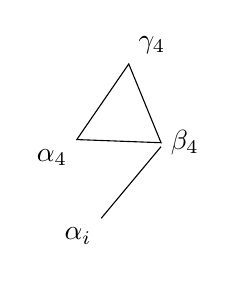
\begin{tikzpicture}[scale=1]
\draw (0,0) node[below left] {$\alpha_4$} -- (.66,.96) node[above right] {$\gamma_4$} -- (1.07,-.04) node[right] {$\beta_4$} -- cycle;
\draw (1.07,-.09) -- (.31,-1) node[below left] {$\alpha_i$};
\end{tikzpicture}}

% l. 5
\uline{Lemme} 9

% ll. 6–8
\diagram{\(\displaystyle\mathrm{III}\left\{\begin{array}{llll}
\alpha_i\ \text{lié à}&\beta_j,\gamma_j,\unsure{\beta'_i},\gamma'_i\ (1\leq i\ne j\leq3)&\text{non à}&\beta'_j,\gamma'_j,\beta_i,\gamma_i\\
\beta_i\ \text{lié à}&\gamma_j,\alpha_j,\unsure{\gamma'_i},\alpha'_i\ (\rule{.7cm}{.35pt})&\rule{.85cm}{.35pt}&\gamma'_j,\alpha'_j,\gamma_i,\alpha_i\\
\gamma_i\ \rule{.8cm}{.35pt}&\alpha_j,\beta_j,\alpha'_i,\beta'_i\ \rule{.7cm}{.35pt})&\rule{.85cm}{.35pt}&\alpha'_j,\beta'_j,\alpha_i,\beta_i.
\end{array}\right.\)}

% ll. 9–11
\diagram{\(\displaystyle\mathrm{III}'\left\{\begin{array}{llll}
\alpha'_i\ \text{lié à}&\beta'_j,\gamma'_j&--&--\\
--&&--&--\\
--&&--&\rule{.38cm}{.35pt}
\end{array}\right.\)}

% ll. 12–14
Il suffit de voir que $\alpha_1$ lié à $\beta_2,\deleted{\beta_3}\beta_3$ \inserted{non à $\beta_1$}. Or

% ll. 13–14 displayed comparison
\[
\begin{aligned}
\alpha_4\ \text{lié à}&\qquad\beta'_1,\beta'_2,\beta'_3,\beta_4\qquad(\text{lemme }8)\\
\alpha_1\ \text{lié à}&\qquad ?\qquad ?\qquad ?\qquad\beta_4
\end{aligned}
\]

% ll. 15–17
\deleted{Donc} l'ens des coïncidences entre $\unsure{w_v(\alpha_1)|\omega_v(\alpha_1)}$ et $w_v(\alpha_4)$ doit être ds la partition $(1,4)(2,3)$, \unsure{ça doit être|ça donc être|se donc être} \deleted{$\beta_4$} $(1,4)$ puisqu'il contient 4, donc

% l. 18
\[
\alpha_1\ \text{lié à}\qquad\beta'_1,\beta_2,\beta_3,\beta_4\qquad\text{cqfd.}
\]

% ll. 19–21
\uline{Conséquence} : $S$ est déterminé par les conditions de départ, à isom. près. \deleted{\illegible{2}} C'est donc un graphe cubique

% bottom centre
\begin{center}cqfd\end{center}

% bottom right
\margin{TSVP}
% archive sheet number: 10
\scanpage{12}

% ll. 1–2
\mspage{\textcircled{10}}
De plus, on trouve ceci :

Considérons les \deleted{diagrammes}\inserted{graphes} suivants

% upper half, graph and count columns
\diagram{\scriptsize\setlength{\arraycolsep}{2pt}\(\displaystyle\begin{array}{clll|l}
&D_0=\varnothing&&&1\\
\cap&\text{\textcircled{$D_1$}}=&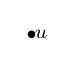
\begin{tikzpicture}[x=.65cm,y=.57cm,baseline=-.4ex,every node/.style={font=\scriptsize,inner sep=.9pt}]
\fill (0,0) circle (1.4pt) node[right] {$u$};
\end{tikzpicture}&\text{pt}&27=3^3.\\
\cap&D_2=&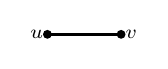
\begin{tikzpicture}[x=.65cm,y=.57cm,baseline=-.4ex,every node/.style={font=\scriptsize,inner sep=.9pt}]
\draw[very thick] (0,0) node[left] {$u$}--(1.44,0) node[right] {$v$};\fill (0,0) circle(1.6pt) (1.44,0) circle(1.6pt);
\end{tikzpicture}&\text{arête}&27.10=2.3^3.5=270\\
\cap&\text{\textcircled{$D_3$}}=&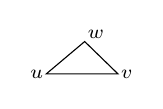
\begin{tikzpicture}[x=.65cm,y=.57cm,baseline=-.4ex,every node/.style={font=\scriptsize,inner sep=.9pt}]
\draw (0,0) node[left] {$u$} -- (.75,.72) node[above right] {$w$} -- (1.4,0) node[right] {$v$} -- cycle;
\end{tikzpicture}&\text{triangle}&27.10.1=2.3^3.5=270\\
\cap&D_4=&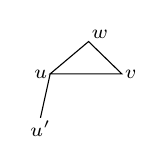
\begin{tikzpicture}[x=.65cm,y=.57cm,baseline=-.4ex,every node/.style={font=\scriptsize,inner sep=.9pt}]
\draw (0,0) node[left] {$u$} -- (.75,.72) node[above right] {$w$} -- (1.4,0) node[right] {$v$} -- cycle;\draw (0,0)--(-.19,-.98) node[below] {$u'$};
\end{tikzpicture}&\text{\deleted{triangle}\inserted{balai}.}&27.10.1.8=2^4.3^3.5=2160\\
\cap&D_5=&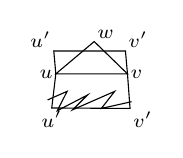
\begin{tikzpicture}[x=.65cm,y=.57cm,baseline=-.4ex,every node/.style={font=\scriptsize,inner sep=.9pt}]
\draw (0,0) node[left] {$u$} -- (.75,.72) node[above right] {$w$} -- (1.4,0) node[right] {$v$} -- cycle;\draw (0,0)--(-.04,.51) node[above left] {$u'$} -- (1.36,.51) node[above right] {$v'$} -- (1.4,0);
\draw (0,0)--(-.08,-.76) node[below] {$u'$}--(1.45,-.77) node[below right] {$v'$}--(1.4,0);
\draw (-.16,-.58)--(.22,-.39)--(.03,-.82)--(.62,-.47)--(.33,-.80)--(1.15,-.39)--(.89,-.77)--(1.48,-.62);
\end{tikzpicture}&\text{préprisme (triangulaire)}&27.10.1.8.4=2^6.3^3.5=8640\\
\cap&D_6=&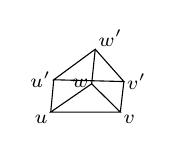
\begin{tikzpicture}[x=.65cm,y=.57cm,baseline=-.4ex,every node/.style={font=\scriptsize,inner sep=.9pt}]
\draw (0,0) node[below left] {$u$} -- (.8,.63) node[left] {$w$} -- (1.36,0) node[below right] {$v$} -- cycle;
\draw (.06,.72) node[left] {$u'$} -- (.87,1.4) node[above right] {$w'$} -- (1.43,.68) node[right] {$v'$} -- cycle;
\draw (0,0)--(.06,.72) (.8,.63)--(.87,1.4) (1.36,0)--(1.43,.68);
\end{tikzpicture}&\text{prisme (triangulaire)}&27.10.1.8.4.1=2^6.3^3.5=8640\\
\cap&\substack{\deleted{\unsure{D_7}}=\\\text{\textcircled{$D_7$}}}&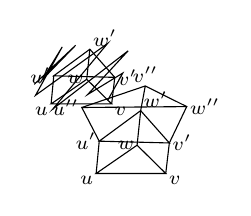
\begin{tikzpicture}[x=.65cm,y=.57cm,baseline=-.4ex,every node/.style={font=\scriptsize,inner sep=.9pt}]
\begin{scope}[shift={(-.88,1.55)},scale=.87]\draw (0,0) node[below left] {$u$} -- (.8,.63) node[left] {$w$} -- (1.36,0) node[below right] {$v$} -- cycle;
\draw (.06,.72) node[left] {$u'$} -- (.87,1.4) node[above right] {$w'$} -- (1.43,.68) node[right] {$v'$} -- cycle;
\draw (0,0)--(.06,.72) (.8,.63)--(.87,1.4) (1.36,0)--(1.43,.68);
\draw (-.38,.5)--(.55,1.5)--(-.20,.62)--(.25,1.46)--(-.35,.22)--(1.27,1.55)--(.04,-.13)--(1.73,1.36)--(.82,.24)--(1.61,.79)--(1.27,.09);\end{scope}
\draw (0,0) node[below left] {$u$} -- (.8,.63) node[left] {$w$} -- (1.36,0) node[below right] {$v$} -- cycle;
\draw (.06,.72) node[left] {$u'$} -- (.87,1.4) node[above right] {$w'$} -- (1.43,.68) node[right] {$v'$} -- cycle;
\draw (0,0)--(.06,.72) (.8,.63)--(.87,1.4) (1.36,0)--(1.43,.68);
\draw (.06,.72)--(-.28,1.47) node[left] {$u''$} -- (1.77,1.49) node[right] {$w''$} -- (1.43,.68);
\draw (-.28,1.47)--(.96,1.95) node[above] {$v''$} -- (1.77,1.49) (.96,1.95)--(.87,1.4);
\end{tikzpicture}&\text{bitriangle}&27.10.1.8.4.1.1=2^6.3^3.5=8640
\end{array}\)}

% ll. 11–12
Soit $\inserted{\mathrm{Pl}_i=}\mathrm{Pl}(D_i,C)$ l'ens des plongements \inserted{(``pleins'')} de $D_i$ dans $C$, $W=\operatorname{Aut} C$, $G_i=\operatorname{Aut}D_i$. Alors

% l. 13
\unsure{b)|c)|\deleted{b)}c)} Les $\mathrm{Pl}(D_i,C)$ sont des espaces homogènes (non vides) sous $G$

% ll. 14–16
a) Les morphismes $\mathrm{Pl}(D_{i+1},C)\mathbin{-}\mathrm{Pl}(D_i,C)$ $(0\leq i\leq6)$ transposés des inclusions $D_i\subset D_{i+1}$ sont surjectifs Ce sont des rev. d'ordres respectifs $27,10,1,8,4,1,1$

% ll. 17–18
b) (Par conséquent) les cardinaux des $\mathrm{Pl}_i$ sont les nbs marqués dans la colonne de droite.

% ll. 18–21
c) Par suite le \unsure{cardinal|cardinalx|cardinaux} \deleted{\unsure{des}} de l'ens \inserted{$\operatorname{Conf}_{D_i}(C)$} des sous-graphes \inserted{pleins} de $C$ \deleted{$\operatorname{Conf}_{D_i}(C)$} de type $D_i$ (s'identifiant à $\mathrm{Pl}_i/G_i$) est donné par $\operatorname{card}\mathrm{Pl}_i/\operatorname{card}G_i$, qui est

% left of assertions into bottom margin
\figure{\begin{tikzpicture}[x=.7cm,y=.48cm]
\draw[->] (1,6.7) .. controls (-.2,4.7) and (.16,2.6) .. (.35,2.2) .. controls (.6,-1) and (.52,-4.8) .. (1.05,-5.1);
\draw[->] (.26,3.38)..controls (.32,2.73) and (.52,2.26)..(1.11,2.18);
\end{tikzpicture}}

% bottom table, rows D0–D7
\diagram{\scriptsize\setlength{\arraycolsep}{2pt}\(\displaystyle\begin{array}{llcll}
\operatorname{Conf}_{D_0}\ {-}&1&--&\operatorname{Aut}D_0&e\\
\operatorname{Conf}_{D_1}&27&--&\operatorname{Aut}D_1&e\\
\operatorname{Conf}_{D_2}&27.10:2=135&---&\operatorname{Aut}D_2&\unsure{\mathfrak S|\mathcal S}_2\\
\operatorname{Conf}_{D_3}&27.10.1:6=45&--&\operatorname{Aut}D_3&\mathfrak S_3\\
\operatorname{Conf}_{D_4}&27.10.1.8:2=2^3.3^3.5=1080&--&\operatorname{Aut}D_4&\mathfrak S_2\\
\operatorname{Conf}_{D_5}&27.10.1.8.4:2=2^5\,3^3\,5=4320&--&\operatorname{Aut}D_5&\mathfrak S_2\\
\operatorname{Conf}_{D_6}&27.10.1.8.4.1:12=2^4\,3^2\,5=720&--&\operatorname{Aut}D_6&\mathfrak S_2\times\mathfrak S_3\\
\operatorname{Conf}_{D_7}&27.10.1.8.4.1.1:72=2^{3}.3.5=120&\cdots-&\operatorname{Aut}D_7&\unsure{\mathfrak S_2.(\mathfrak S_3\times\mathfrak S_3)}
\end{array}\)}
% archive sheet number: 11
\scanpage{13}

% ll. 1–3
\mspage{\textcircled{\scriptsize 10 bis}}
d) Le stabilisateur d'un élément de $\mathrm{Pl}_6$ \deleted{dans} \inserted{(ou, ce qui revient} au $=$, de $\mathrm{Pl}_5$ ou $\mathrm{Pl}_7$) dans $W$ est isomorphe à $\unsure{\mathfrak S|\mathcal S}_3$ (via l'opération sur l'ens $I$ \inserted{de cardinal 3} des éléments de

% ll. 4–9
\deleted{$E(u)^*=E(u)-\{v,w\}$} $E(u)^*=E(u)-\{v,w\}$ qui sont $\ne u'$, \deleted{non liés à $\unsure{u'|v'|v}$} et liés à $v'$, i.e. des él. de $E(u)-\{v\deleted{\unsure{,w}},u',\unsure{w}\}$ qui sont liés à $v'$, i.e. $I=E(u)\cap E(v')-\{u',v\}$. On voit \inserted{donc} que cet $I$ est can. is. aux $(9.4):2=18$ ensembles analogues tels que $E(v'')\cap E(w')-\{u'',w'\}$ etc $\dots$ $\}$. Donc $W$ est de cardinal égal à $\operatorname{card}\mathrm{Pl}_6\,.6$ \unsure{$\Rightarrow$} i.e.

% l. 10
\[
\operatorname{Card}W=2^7.3^4.5=51840
\]

% centred rule
\begin{center}\rule{1.15cm}{.35pt}\\[-1.2ex]\rule{.95cm}{.35pt}\end{center}

% below rule, left
\deleted{\unsure{Graphe|Compte}}\\
\deleted{Complexe cubique}
% archive sheet number: 12
\scanpage{14}

% ll. 1–4
\mspage{\textcircled{11}}
La catégorie formée des $S$, avec un triangle $I\subset S$ et un triangle $I'\subset S$ disjoint du précédent, (pour les iso) équivaut à celle des couples $(I,\Pi)$ de deux ens. de \unsure{cardinal.|cardinl.|cardinal} 3.

% ll. 5–7
À un \inserted{tel} couple on associe

% ll. 5–6, indented equations
\[
\begin{aligned}
S&=\underset{\substack{\ni\\u}}{I}
\sqcup(I\sqcup I)\sqcup I\times\Pi\times\omega(I)\\
&\hspace{8mm}u\longmapsto\alpha_4(u),\alpha'(u)\\
&\inserted{=(I\times\{0,1,2\})\sqcup(I\times\Pi\times\omega(I))}
\end{aligned}
\]

% l. 7
où $\omega(I)\inserted{\subset\unsure{\mathfrak S|\mathcal S}_I}$ est l'ens \inserted{(de cardinal 2)} des ordres circulaires sur $I$.

% cancelled sketch above conditions
\figure{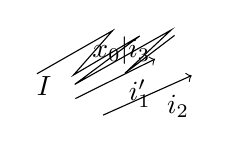
\begin{tikzpicture}[scale=.75]
\node at (0,0) {$I$};\draw[->] (.53,-.22)--(1.88,.45);\draw[->] (1,-.50)--(2.50,.17);
\node at (1.31,.59) {$\unsure{x_0|i_3}$};\node at (1.62,-.14) {$\unsure{i'_1}$};\node at (2.27,-.35) {$\unsure{i_2}$};
\draw (-.12,.2)--(1.16,.93)--(.5,.18)--(1.62,.84)--(.52,.02)--(2.15,.94)--(1.37,.21)--(2.21,.85);
\end{tikzpicture}}

% same line, to right of sketch
\deleted{Si $i\in I$, $i$ est lié à}

% ll. 9–12
$(i,\nu)$ et $(\unsure{j'|j},\mu)$ \inserted{(distincts)} sont liés ssi $i=j$ \uline{ou} $\nu=\mu$

% second condition
\[
\begin{aligned}
(i,\nu)\text{ et }(j,\pi,\rho)\quad &\deleted{\unsure{\text{sont}}}\ \text{liés }\deleted{\unsure{\text{ssi}}}\quad\text{si}\\
&\text{dans les cas }\left\{\begin{array}{ll}
i=\deleted{\unsure{j'}}j &\nu=0\\
i\ne j&\left\{\begin{array}{l}\nu=1,\ j=\rho i\\ \nu=2,\ i=\rho j\end{array}\right.
\end{array}\right.
\end{aligned}
\]

% third condition
\[
\begin{aligned}
(j,\pi,\rho)\text{ et }(j',\pi',\rho')&\ \inserted{\text{distincts}}\quad\text{liés}\\
(\underset{I}{\uparrow}\ \underset{\Pi}{\uparrow}\ \underset{\omega(I)}{\uparrow}
\qquad\text{id})&\quad\text{dans les cas }\left\{\begin{array}{ll}
j=j'&\pi=\pi',(\rho\ne\rho')\\
j\ne j'&\left\{\begin{array}{ll}i\ne j,&\rho=\rho'\\i'=j&\rho\ne\rho'\end{array}\right.
\end{array}\right.
\end{aligned}
\]

% left of three conditions
\figure{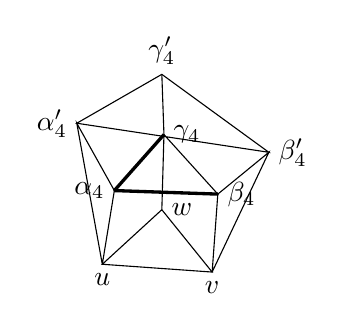
\begin{tikzpicture}[scale=.9]
\coordinate (u) at (.2,0);\coordinate (v) at (1.75,-.11);\coordinate (w) at (1.04,.77);
\coordinate (a) at (.37,1.04);\coordinate (b) at (1.83,.99);\coordinate (g) at (1.07,1.83);
\coordinate (aa) at (-.16,1.99);\coordinate (bb) at (2.55,1.58);\coordinate (gg) at (1.04,2.68);
\draw (u)--(w)--(v)--cycle (a)--(g)--(b)--cycle (aa)--(gg)--(bb)--cycle;
\draw (u)--(a)--(aa)--(u) (v)--(b)--(bb)--(v) (w)--(g)--(gg); \draw[very thick] (a)--(g) (a)--(b);
\node[below] at (u) {$u$}; \node[below] at (v) {$v$}; \node[right] at (w) {$w$};
\node[left] at (a) {$\alpha_4$}; \node[right] at (b) {$\beta_4$}; \node[right] at (g) {$\gamma_4$};
\node[left] at (aa) {$\alpha'_4$}; \node[right] at (bb) {$\beta'_4$}; \node[above] at (gg) {$\gamma'_4$};
\end{tikzpicture}}

% ll. 14–20
L'autom $\sigma$ conserve $I\times[0,1,2]$ et son complémentaire, et agit \deleted{\unsure{sur}} \unsure{en permu|sur le premier} \deleted{via} l'identité sur $I$, et la permutation entre 1 et 2 sur l'autre facteur ; sur $I\times\Pi\times\omega(I)$ il agit par permutation des deux \deleted{facteurs} élmts de $\omega(I)$ (et l'identité sur $I\times\Pi$).

% left beside action, two columns of jottings
\margin{$\underbrace{\unsure{i\,u|u}\overset{\text{ou}}{/}\alpha_4\overset{\text{ou}}{/}\alpha'_4}$ \quad $\unsure{\alpha_i},\alpha'_{\unsure{i}}$\\
$(\deleted{\unsure{u}},\underset{1\leq{i}\leq3}{\deleted{\unsure{\pi}}\pi},\rho)\ \inserted{\unsure{\alpha'_u}}$\quad $\beta_j\quad\beta'_j$\\
$1\leq i,j\leq3$\\ $\alpha_u$ ou $\alpha'_u$}

% ll. 21–22
\[
\begin{aligned}
&I\sqcup(I\times\varepsilon)\sqcup(I\times\Pi\times\varepsilon\times\omega(I)/\mathbb F_2)\\
&(I\times J)\sqcup
\end{aligned}
\]

% bottom left, crossed table
\diagram{\(\displaystyle\deleted{\begin{array}{lll}
\alpha_4&\beta_4&\gamma_4\\
\alpha'_4,&\beta'_4,&\gamma'_4,\\
\alpha_1,&\beta_2,&\gamma_3\\
\unsure{\alpha_1},&\unsure{\beta'_4},&\unsure{\gamma'_4}
\end{array}}\)}
% archive sheet number: 13
\scanpage{15}

% ll. 1–2
\mspage{\textcircled{12}}
\uline{Proposition} $G$ groupe abélien (pour simplifier), $V=G\otimes_{\mathbb Z}\mathbb F_2$, $\varepsilon$ un $\mathbb F_2$ vectoriel, $\unsure{\Gamma|\mathscr T}=\Psi(G)=\operatorname{Ker}(G\times G\times G\xrightarrow[(x,y,z)\mapsto x+y+z]{}G)$,

% upper right, beside lines 2–5
\margin{$p_i:\Psi(G)\to G$ induit par $\mathrm{pr}_i$ $(1\leq i\leq3)$\\
$N_i=\operatorname{Ker}p_i\xleftarrow[\alpha_i]{\sim}G$\\
\deleted{$\unsure{g\mapsto(g,\widehat 0,g)|\{(x,\widehat x,x\}}$}}

% ll. 3–4
a) Pour tte extension centrale \deleted{\unsure{de|$E_0$}} :

% l. 4 displayed sequence
\[
1\longrightarrow\varepsilon\mathbin{-} E_0\longrightarrow G\mathbin{-}1
\]

% ll. 5–8
considérons $\Psi(E_0)=p_1^*(E_0)\wedge p_2^*(E_0)\wedge p_3^*(E_0)=\widetilde\Gamma$ (produit de Baer d'extensions de $\deleted{\unsure{\Psi_2}}\Gamma$ par $\varepsilon$, images inv de l'ext. $E_0$ (\deleted{\unsure{de}} $G$ par $\varepsilon$) par les $p_i$). Comme $p_j\alpha_i=\left\{\begin{array}{ll}0&\text{si }i=j\\ \mathrm{id}_G&\text{si }i\ne j\end{array}\right.$, on trouve que $\alpha_i^*(\widetilde E)$ est splitté canoniquement.

% ll. 9–10
d'où

% ll. 9–10, diagram
\diagram{\begin{tikzcd}[ampersand replacement=\&,column sep=1.6em,row sep=1.25em]
1 \arrow[r,dash]\& \varepsilon \arrow[r]\& \widetilde E \arrow[r]\& \Gamma \arrow[r,dash]\&1\\
\&\&\& G\arrow[ul,"\rho_i"]\arrow[u,"\alpha_i"']\&
\end{tikzcd}}

% ll. 11–12
Ceci posé, si
\[
q:\dot V\longrightarrow\varepsilon
\]

% ll. 13–14
est l'application quadratique qui définit la classe de l'extension $E_0$, on a pour $g\in G$

% l. 15
\[
\rho_1\deleted{\unsure{\alpha_1}}(g)\rho_{\unsure{2|1}}\deleted{\unsure{\alpha_2}}(g)\rho_3\deleted{\alpha_3}(g)=q(\dot g)
\]

% l. 16
où $\dot g\in V$ est la classe de $g\in\unsure{K|G}$ ds $V=G/2\unsure{C|G}$.

% ll. 17–23
b) Toute \inserted{syst. $(\widetilde E,\rho_1,\rho_2,\rho_3)$ d'une} extension \inserted{centrale} $E$ de $\Gamma$ par $\varepsilon$ et de relèvements $\rho_1,\rho_2,\rho_3$ de $\alpha_1,\alpha_2,\alpha_3$ provient d'une extension $E_0$ de $G$ par $\varepsilon$, déterminée à isom (non unique) près --- sa classe $q\in\mathrm{Quad}_{\mathbb Z}(G,\varepsilon)\simeq\mathrm{Quad}_{\mathbb F_2}(V,\varepsilon)$ est donnée par la formule précédente. La catégorie \inserted{(pour les iso)} des \deleted{triples} syst. $(\widetilde\Gamma,\rho_1,\rho_2,\rho_3)$ est \uline{rigide} i.e. tout autom est l'identité (donc tt autom. de l'ext. $E_0$ induit l'identité sur \inserted{l'ext} $\Psi(E_0)$ \dots.)
% archive sheet number: 14
\scanpage{16}

% head
\mspage{\textcircled{13}}
c) Conditions équivalentes

% condition (i)
(i) \inserted{$2G=0$ i.e. $G\simeq V$, et} $q(u)\ne0$ pour \deleted{\unsure{$u\ne0$}} $u\in V^*=V-\{0\}$

% condition (ii), ll. 3–6
(ii) Posant $\widetilde P_i=\widetilde E/\rho_i(G)$, \deleted{\unsure{la fon Pon|la fam Posons}} et $\widetilde p_i:\widetilde E\unsure{\longrightarrow|\mathbin{-}}\widetilde P_i$, si $x_1,x_2,x_3\in\widetilde\Gamma$ sont tels que $p_1(\widetilde x_2)=p_1(\widetilde x_3)$, $p_{\unsure{2|3}}(\widetilde z_3)=p_2(\widetilde x_{\unsure{1|3}})$, $p_3(\widetilde x_1)=p_3(\widetilde x_2)$, alors $\widetilde x_{\unsure{1|2}}=\widetilde x_2=\widetilde x_3$.

% condition (iii), ll. 7–8
(iii) Si $\widetilde z_1\in\rho_1(G)$, $\widetilde z_2\in\rho_2(G))$, $\widetilde z_3\in\rho_3(G)$ sont tels que $\widetilde z_1\widetilde z_2\widetilde z_3=0$, alors $\widetilde z_1=\widetilde z_2=\widetilde z_3=1$

% condition (iv), ll. 9–10
(iv) Si $g\in G$ est tel que $\rho_1(g)\rho_2(g)\rho_3(g)=1$, alors $g\unsure{=|\equiv}1$

% conclusion, ll. 11–14
De plus, pour $G,\varepsilon$ fixés avec $\varepsilon\unsure{\ne|=}\mathbb F_2$, $\exists$ une $\widetilde\Gamma$ \deleted{ext} avec ces propriétés \unsure{sss|ssi} $2G=0$ i.e. $G\simeq V$, $\operatorname{rg}_{\mathbb F_2}V\leq2$ (et cette extension est unique à isom unique près).
% archive sheet number: 15
\scanpage{17}

% l. 1
\mspage{\textcircled{\scriptsize 13 bis}}
$S$ graphe \inserted{$\ne\varnothing$} tel que \deleted{l'ens de ses \unsure{arêtes est} \illegible{2} et}

% ll. 2–3
\[
\begin{aligned}
\text{a)}\quad&\forall x,y\in S\text{ liés},\quad\exists!z\in S\text{ tel que }z\text{ soit lié à }x\text{ et }y\\
\text{b)}\quad&\exists\,\nu\in\mathbb N^*\text{ tel que }\forall s\in S,\quad\operatorname{Card}\underbrace{E(s)}_{\{t\in S\mid t\text{ lié à }s\}}=\nu
\end{aligned}
\]

% ll. 4–6
\deleted{c)} \uline{Lemme 1} \inserted{$\nu$ est pair, et} On a $\operatorname{card} S\geq3(\nu-1)$. On a égalité \unsure{sss|ssi} $\forall$ \inserted{(\unsure{resp.|ou|il en} $\exists$)} triangle $T=\{x,y,z\}$ de $S$, \deleted{\unsure{à|a}} tt élément de $S^{\unsure{\prime|*}}=S-T$ est lié à un (et un seul) élément de $T$.

% ll. 7–10
\[
\begin{aligned}
\nu&=2(\mu+1)&2\\
\operatorname{card}S&=3(2\mu+1)&\operatorname{card} S-\operatorname{card}(E(s))\inserted{-1}&=\operatorname{card}(S-E(s)\inserted{-\{s\}})=4\mu\deleted{\unsure{+1}}\\
&&4\mu&\leq2^{\mu+1}\qquad\mu\leq2^{\mu-1}\\
&&&\deleted{\unsure{2\mu+1}}
\end{aligned}
\]

% left below computation, small triangle
\figure{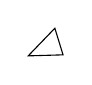
\begin{tikzpicture}[scale=.65]\draw (0,0)--(.52,.54)--(.68,.02)--cycle;\end{tikzpicture}}

% next to small triangle, looped graph
\figure{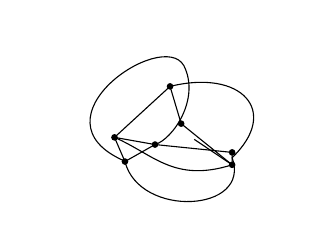
\begin{tikzpicture}[scale=.83]
\draw (0,0)--(.85,.78)--(1.02,.21)--(1.8,-.42)--(1.8,-.23)--(.62,-.11)--cycle;
\draw (.85,.78)..controls (1.95,1.05) and (2.54,.40)..(1.8,-.31) ..controls (2.10,-1.15) and (.38,-1.24)..(.16,-.37)--(0,0);
\draw (.15,-.36)..controls (-1.32,.28) and (.73,1.67)..(1.06,1.10)..controls (1.32,.59) and (.89,-.03)..(.62,-.11)--(.16,-.37);
\draw (0,0)..controls (.60,-.26) and (.91,-.70)..(1.8,-.42) (1.22,-.03)--(1.8,-.42);
\foreach \x/\y in {0/0,.85/.78,1.02/.21,.62/-.11,.16/-.37,1.8/-.42,1.8/-.23}{\fill (\x,\y) circle (1.45pt);}
\end{tikzpicture}}

% lower of three drawings, before fold
\figure{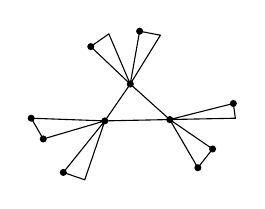
\begin{tikzpicture}[scale=.85]
\draw (0,0)--(.38,.55)--(.97,.02)--cycle;
\draw (0,0)--(-1.10,.04)--(-.92,-.27)--cycle (0,0)--(-.62,-.77)--(-.30,-.88)--cycle;
\draw (.38,.55)--(-.21,1.11)--(.06,1.30)--cycle (.38,.55)--(.52,1.34)--(.83,1.28)--cycle;
\draw (.97,.02)--(1.92,.26)--(1.95,.04)--cycle (.97,.02)--(1.61,-.42)--(1.39,-.70)--cycle;
\foreach \x/\y in {0/0,.38/.55,.97/.02,-1.1/.04,-.92/-.27,-.62/-.77,-.21/1.11,.52/1.34,1.92/.26,1.61/-.42,1.39/-.70}{\fill (\x,\y) circle (1.5pt);}
\end{tikzpicture}}
% archive sheet number: 16
\scanpage{18}

% top, ms folio
\mspage{\textcircled{14}}

% l. 1, heading
\uline{Graphes cubiques \inserted{$C$} à sommet marqué} $u$

% ll. 2–6
Revient à la donnée d'un ens $\unsure{P|Q}_u$ de cardinal $5$ (l'ens des $5$ triangles de sommet $u\unsure{\}|)}$, ou encore des $5$ couples de pts mutuellt liés de $E(u)$), et d'un torseur $P$ sous $\Psi=\Psi(P_u,\mathbb F_2):\operatorname{Ker}\bigl(\mathbb F_2^{P_u}\xrightarrow[\inserted{(x_i)_{i\in I}\mapsto\sum x_i}]{}\mathbb F_2\bigr)$. \deleted{Ce torseur} \inserted{On \unsure{réconstitue|reconstruit|reconstitue}}

% ll. 7–9
$E(u)$ comme l'ens somme des $P\wedge_\Psi(\mathbb F_2,p_i)$, où les $p_i:\Psi\longrightarrow\mathbb F_2$ \inserted{$(i\in E)$} sont induits par les projections $\mathbb F_2^{P_u}\xrightarrow{\mathrm{pr}_i}\mathbb F_2$ $(i\in P_u)$, et $C-E(u)$ comme $P$, donc

% l. 10
\[
 C\simeq\Bigl(\coprod_{i\in E}P\wedge_\Psi(\mathbb F_2,p_i)\Bigr)\amalg P\amalg\{u\}.
\]

% ll. 10–20
La \unsure{recette|vieille} pour ce dictionnaire est la suivante: $E(u)$ est un ens de cardinal $10$ muni d'un autom involutif d'ordre $2$ ss pt fixe (car tt él de $E(u)$ est lié à un et un seul él. de $E(u)$, grâce à l'axiome du triangle), or une telle structure est déterminée par un ens $P_u$ de cardinal $5$ ($P_u=E(u)/\sigma$) et une famille d'ens à $2$ él. i.e. de $\mathbb F_2$ torseurs, paramétrés par $P_u$ -- i.e un torseur $Q$ sous $(\mathbb F_2)^{P_u}$.

% ll. 20–24
D'autre part, tt $x\in C-E(u)$ définit une partie de $E(u)$ -- savoir $E(x)\cap E(u)$ -- telle que \deleted{\unsure{sa}} intersection avec tte classe sous $\{e,\sigma\}$ i.e. tte fibre de $\overset{\inserted{=\widetilde Q_u}}{E(u)}\longrightarrow\unsure{Q|P}_u$ i.e. tte orbite $\subset E(u)$, soit de cardinal $1$.

% ll. 24–28
Or l'ens de ces parties n'est autre que $Q$ (qui est de cardinal $2^5=32$) alors que $C-E(u)$ est de card $16=32/2$. On trouve que $C-E(u)\longrightarrow Q$ est \uline{injectif}, et son image \inserted{$P$} est un torseur sous $\Psi\subset\mathbb F_2^{P_u}$, $\bigl(\Psi=\operatorname{Ker}(\mathbb F_2^{P_u}\longrightarrow\mathbb F_2)\bigr)$ -- donc on a sur $Q$ une reconstitution du groupe

% bottom left
% archive sheet number: 17
